\chapter{Ergebnisse}

%-------------------

\section{Auswertung der Resultate}
\label{sec:3ergebnisse}

Es werden in diesem Kapitel die erhaltenen Resultate mit der Variante des MST behandelt. Diese werden mit den Ergebnissen des Steiner Baums verglichen.


\vspace{1cm}

\section{Resultate Steiner Baum}
\label{sec:3 ergebnisse}

Das Programm RTR\_R2008a verwendet zur Ermittlung der optimalen Trassierung einen Steiner Baum, welcher in Kapitel 2.2.2 
kurz beschrieben wird.
Mit diesem wird der kostenoptimierte Weg für eine Trassierung als Graph abgebildet.
Die Modellierung von nicht redundanten Netzwerktrassierungen (Bäumen) erfolgt mittels Steiner Bäumen. Diese Probleme werden mit Hilfe von primaldualen
Approximationsmethoden gelöst.
Trassenredundante Netzwerkstrukturen werden als Generalized Steiner Baum-Problem modelliert, wobei wiederum primal-duale Approximationsmethoden
oder Augmentierungsansätze zur Lösung der Probleme verwendet werden \cite{tech_rep_1}.

\vspace{1cm}

\section{Resultate MST}
\label{sec:3 ergebnisse}

Wie in Kapitel 2.2.3 erläutert, handelt es sich in dieser Arbeit um einen wissenschaftlichen Versuch
einen Steiner Baum nachzubilden. In Abbildung 3.1 werden die Resultate beider Baumalgorithmen gegenübergestellt. 
Sofort erkennbar ist, dass mit dem MST die Längen in beinahe jedem Wählamtsbereich wesentlich länger sind. Im Durchschnitt ergeben sich um
68,78\% längere Anschlusslängen, als beim Steiner Baum Algorithmus.
Bei genauerer Betrachtung ist erkennbar, dass in nur einem der gewählten Wählamtsbereiche die maximale Anschlusslänge kürzer ausfällt.



\begin{figure}[H]
    \centerline{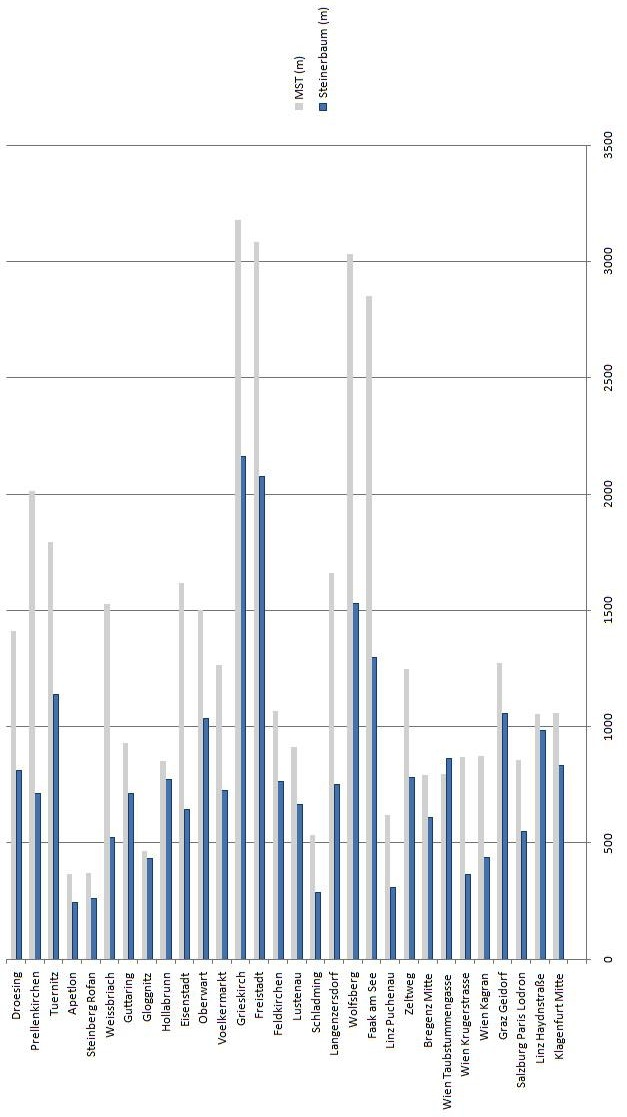
\includegraphics[scale=0.8]{pics/final_mst-steiner}}
    \caption[Gegenüberstellung der Resultate von MST und Steiner Baum]{\label{FiG:Gegenüberstellung der Resultate von MST und Steiner Baum} Gegenüberstellung der Resultate von MST und Steiner Baum in Meter}
\end{figure}

\vspace{1cm}

Um die Ergebnisse besser interpretieren zu können, muss eine statistische Bewertung durchgeführt werden. 

\subsection{Statistische Auswertung der Resultate}
\label{sec:3 ergebnisse}

\vspace{0.3cm}

Die erhaltenen Ergebnisse liegen in einem breit gestreutem Bereich. 
Nun muss ein Bereich definiert werden, in welchem die Anschlusslängen liegen dürfen.
Realisiert wird diese Berechnung, indem ein Konfidenzintervall (darauffolgendes Unterkapitel) berechnet wird.\\
Mit Hilfe von diesem wird eine Unter-und Obergrenze ermittelt. Über- oder unterschreiten die erhaltenen Anschlusslängen (Abbildung 3.1) eines
Wählamtsbereiches den definierten Bereich, werden sie verworfen.

\vspace{0.5cm}

\begin{graybox}
\textbf{\textit{Bemerkung:}} Es ist möglich, dass es zu von uns genannten \textit{Ausreißern} kommt. 
Diese überdurchschnittlich langen Versorgungslängen können entstehen, wenn die Durchquerung eines Gewässers vermieden wird (Kapitel 2.1.4). 
Auch in den Wählamtsbereichen, die für diese Arbeit herangezogen wurden, war einer dieser \textit{Ausreißer} vorhanden.   
Jedoch verfälschen sie in Folge das Resultat und  müssen deshalb ausgeschlossen werden.
\end{graybox}

\vspace{0.5cm}

Beurteilende Statistik hat das Ziel, eine Aussage über eine Grundgesamtheit (Population und Merkmale) zu gewinnen. Dies wird mit Stichproben durchgeführt.   

\vspace{0.5cm}

\begin{graybox}
\textbf{\textit{Definition:}} Eine Stichprobe vom Umfang $n \in N$ ist eine Folge von zufällig gewählten Objekten aus der Population - also eine Folge
von $n$ Zufallsvariablen$~(X_{i})_{i \in N}$\cite{bachhiesl2}.
\end{graybox}

\vspace{1cm}


\subsubsection{ Konfidenzintervall}
\label{sec:3 ergebnisse}

Gesucht wird ein Intervall, um den realisierten Schätzer des Erwartungswertes $\overline x$, sodass der exakte Erwartungswert $\mu$ der Zufallsvariable 
$X$ mit $Q$-prozentiger Wahrscheinlichkeit in diesem Intervall liegt. 
Es wird angenommen, dass die Variablen $X \in N (\mu,\sigma)$ wobei $\mu$ und $\sigma$ unbekannt sind.
Unter Zuhilfenahme einer realisierten Stichprobe $x_{1},...,x_{n}$ vom Umfang $n$, können die unbekannten Parameter geschätzt werden.

\vspace{0.3cm}


Der Erwartungswert $\mu$ kann mit $\overline x$ abgeschätzt werden.

\vspace{0.3cm}

\begin{equation}
\overline x = \frac 1 n  \sum_{i=1}^{n} x_{i}
\end{equation} 

\vspace{0.3cm}

Das erhaltene $\overline x$ entspricht einem realisierten Schätzer des Erwartungswertes $\mu$. 
Nun kann die Standardabweichung $\sigma$ geschätzt werden.

\vspace{0.3cm}

\begin{equation}
s_{\overline x} =\sqrt{ \frac {\sum_{i=1}^{n}(x_{i}-\overline x)^2} {n(n-1)} } 
\end{equation}

\vspace{0.3cm}

Mehrere Stichproben vom Umfang $n$ führen zu mehreren Werten für $\overline x$ und $s_{\overline x}$ und damit auf mehrere Konfidenzintervalle.

\vspace{0.5cm}

\begin{graybox}
\textbf{\textit{Beispiel:}} Q=0.9. Werden 100 Stichproben gezogen so folgen 100 Konfidenzintervalle $K$. Es darf erwartet werden, dass 90 den zu schätzenden
Parameter $\mu$ enthalten und 10  nicht. Man beachte in diesem Zusammenhang: je grösser $Q$ gewählt wird, desto breiter die Intervalle\cite{bachhiesl2}.
\end{graybox}



\vspace{0.3cm}
In dieser Berechnung sind $X$ die maximalen Versorgungslängen (ersichtlich in Abbildung 3.1).
Diese Längen sind die gewählten Stichproben 
$x_{1},...,x_{n}$ mit dem Umfang $n$ (Anzahl der Wählamtsbereiche).

Um das Konfidenzintervall bestimmen zu können, muss ein zweiseitiges Quantil \\der $t_{n-1,\alpha}$-Verteilung bestimmt werden, wobei $n-1$ der 
Freiheitsgrad und $\alpha = Q-1$ die Wahrscheinlichkeit der $t$-Verteilung ist. $Q$ bezeichnen wir auch als Vertrauenswahrscheinlichkeit.
Es wird eine Stichprobe realisiert und ein Konfidenzintervall $KI$ ernannt, wobei $\mu$ und $\sigma$ unbekannt sind.
Das Konfidenzintervall $KI$ für $\mu$ sei mit einer Vertauenswahrscheinlichkeit $Q$ gegeben:

\vspace{0.3cm}

\begin{equation}
KI = \lbrack \overline x - s_{\overline x}t_{\alpha /2,n-1}, \overline x + s_{\overline x}t_{\alpha /2,n-1}\rbrack
\end{equation}

\vspace{0.3cm}

Das Ergebnis des Konfindenzintervalls $~KI~$ für diese Realisierung beträgt:

\begin{equation}
[573,360~m;1024,500~m] 
\end{equation}

Der erste Wert ist die Untergrenze, der zweite gibt die Obergrenze an.
Die Lösung der Dichtefunktion der $t$-Verteilung ergibt $t=2,75$\cite{bronstein}.
Es wurde eine Vertrauenswahrscheinlichkeit von 99\% gewählt. 


\begin{figure}[H]
    \centerline{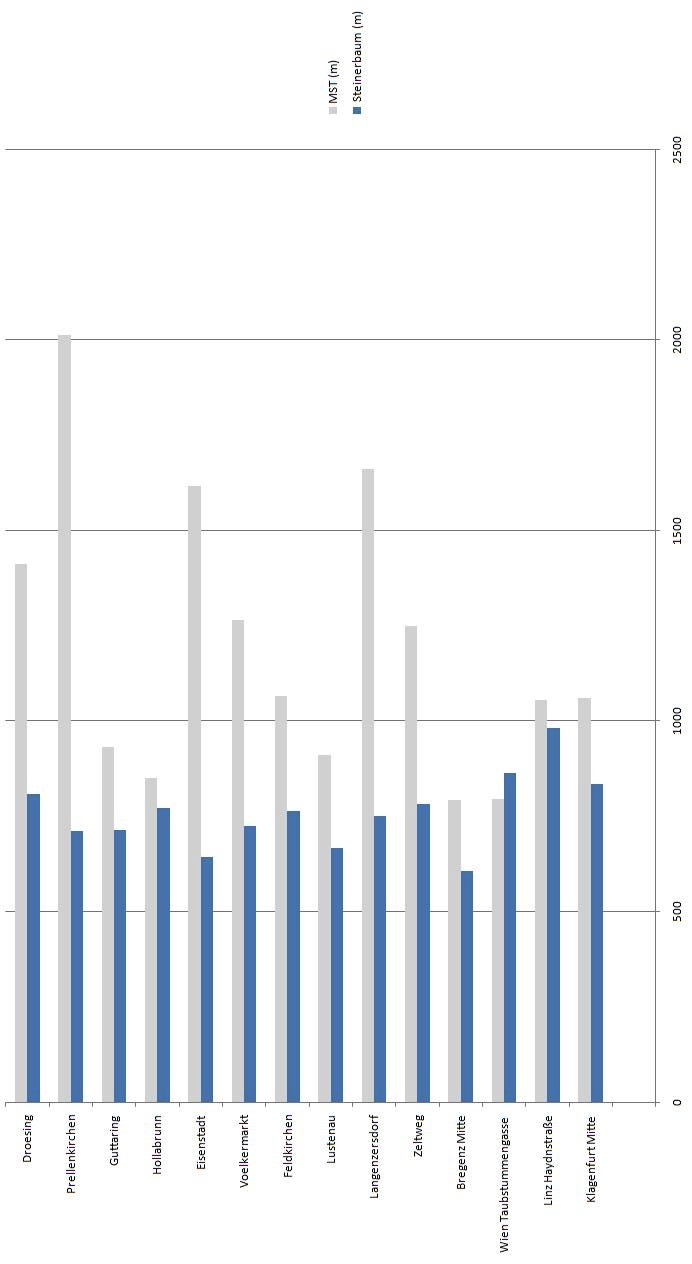
\includegraphics[scale=0.7]{pics/final_final}}
    \caption[Abweichung in gültigen Wahlamtsbereichen]{\label{FiG:Abweichung in gültigen Wahlamtsbereichen}
     Abweichung der im Konfidenzintervall liegenden Wählamtsbereiche}
\end{figure}

